\documentclass[10pt,twocolumn]{article}
\usepackage[letterpaper,margin=0.75in,top=1in,bottom=1in,columnsep=0.25in]{geometry}
\usepackage{times}
\usepackage{amsmath,amssymb}
\usepackage{booktabs}
\usepackage{colortbl}
\usepackage{graphicx}
\usepackage[hidelinks]{hyperref}
\usepackage{xcolor}
\usepackage{fancyhdr}
\usepackage{titlesec}
\usepackage{caption}
\usepackage{pgfplots}
\pgfplotsset{compat=1.17}
\usetikzlibrary{arrows.meta,positioning,calc}
\definecolor{accent}{RGB}{42,101,175}
\definecolor{corrupt}{RGB}{201,109,44}
\definecolor{inkmut}{RGB}{110,118,126}
\definecolor{best}{RGB}{214,238,214}

% ICML-style typography approximations
\titleformat{\section}{\large\bfseries}{\thesection.}{0.5em}{}
\titleformat{\subsection}{\normalsize\bfseries}{\thesubsection.}{0.5em}{}
\titleformat{\subsubsection}{\normalsize\bfseries\itshape}{\thesubsubsection.}{0.5em}{}
\titlespacing*{\section}{0pt}{1.6ex plus .4ex}{0.8ex}
\titlespacing*{\subsection}{0pt}{1.2ex plus .3ex}{0.5ex}
\captionsetup{font=small,labelfont=bf,skip=4pt}
\pagestyle{fancy}
\fancyhf{}
\fancyhead[C]{\small Hardening Mixture-of-Agents: An Evidence-Bound Harness for Specialist Aggregation Pipelines}
\fancyfoot[C]{\small\thepage}
\renewcommand{\headrulewidth}{0.4pt}
\setlength{\abovedisplayskip}{4pt}
\setlength{\belowdisplayskip}{4pt}

\newcommand{\ci}[2]{\ensuremath{[#1,\,#2]}}
\newcommand{\bestcell}{\cellcolor{best}}

\title{\LARGE\bfseries Hardening Mixture-of-Agents:\\ An Evidence-Bound Harness for Specialist Aggregation Pipelines}
\author{\textbf{Sam Bobo}\\ \small Draft v0.2, September 2026}
\date{}

\begin{document}

\twocolumn[
\begin{@twocolumnfalse}
\maketitle
\thispagestyle{fancy}
\begin{center}
\begin{minipage}{0.9\textwidth}
\begin{center}\textbf{Abstract}\end{center}
\small
Mixture-of-Agents (MoA) pipelines route a task through several
proposer models and synthesize their outputs through an aggregator,
and report state-of-the-art results on preference-judged benchmarks.
Every published gain, however, is measured by a preference judge, and
nothing in that evaluation tests whether the aggregator verifies what
it is given, whether proposer caution reaches the reader, or whether a
corrupted proposer corrupts the answer. This paper presents an
evidence-bound harness that hardens the MoA recipe against exactly
those failures. The harness keeps the recipe's proposer-aggregator
structure and its measured preference lift, and adds five mechanisms:
an empirical seating gate, engineered redundancy across proposers,
re-consultation triggered by a mandated artifact rather than by any
model's self-assessment, an out-of-band channel that carries proposer
qualification around the aggregator, and a charter of diagnostics that
may never be optimized. Each mechanism is licensed by a pre-registered
experiment on an auditable MoA instance (7 to 20B local models, more
than fifty registered experiments) that falsified a premise the recipe
depends on: the aggregator adopts a sole-sourced corrupted value at
$0.90$, an instruction to mark uncertainty installs only its named
phrase, order-debiased judges penalize that phrase while rewarding
aggregation, prose transports $0.11$ to $0.33$ of supplied
qualification, and elicited self-assessment predicts behavior at
chance. Under prospective single-factor re-tests, engineered redundancy
halves corrupted-value adoption ($0.900$ to $0.450$), the out-of-band
channel carries $1.000$ of proposer caveats against $0.174$ through
prose and changes reader decisions ($+0.691$ over a matched control),
live re-consultation resolves contested quantities at $0.905$ against
$0.333$, and the seating gate predicts in-pipeline defects ($+0.632$).
Two of the harness's own rationales were demoted by registered tests
and one gate failed twice. Judged head-to-head against the unmodified
pipeline under a two-family order-debiased protocol, the assembled
harness shows no evaluable preference difference: it fixes what the
recipe's evaluation cannot measure at no cost on what it can.
\end{minipage}
\end{center}
\vspace{1.2em}
\end{@twocolumnfalse}
]

\section{Introduction}
\label{sec:intro}

\begin{figure*}[t]
\centering
\resizebox{\textwidth}{!}{%
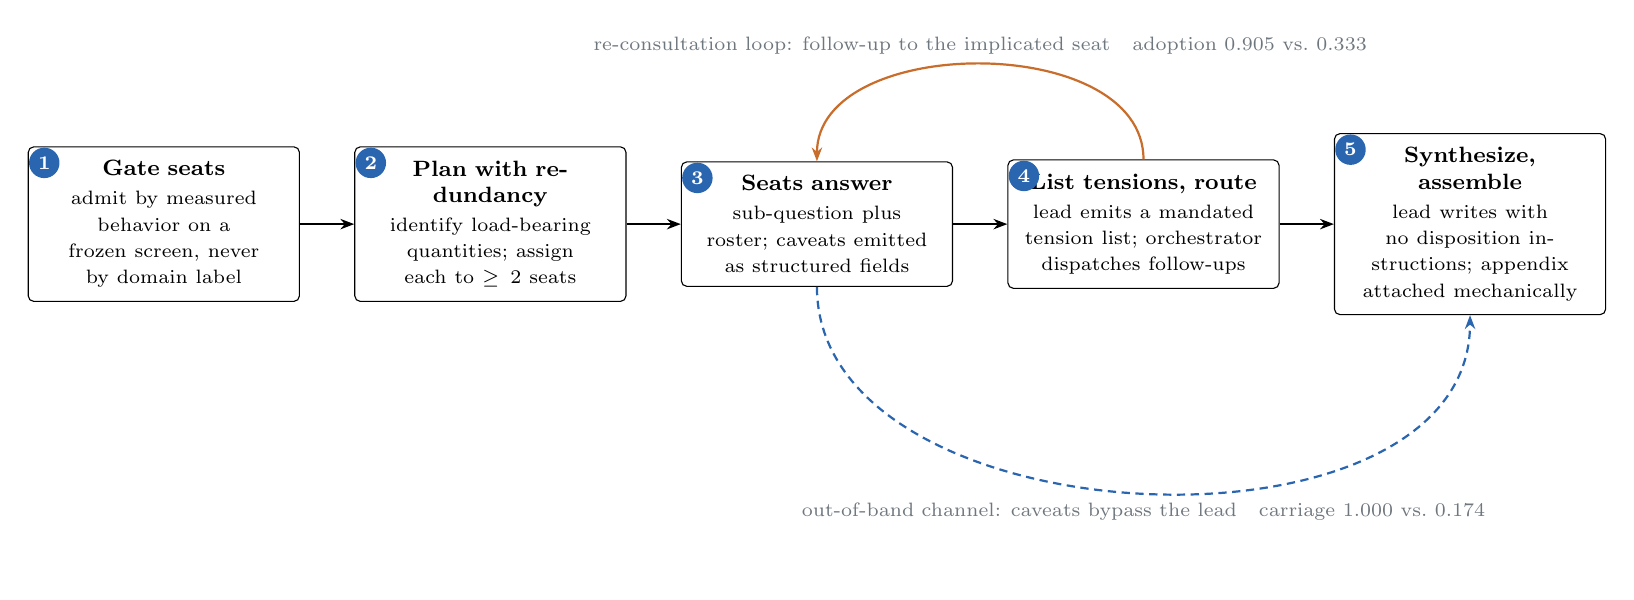
\begin{tikzpicture}[x=1pt,y=1pt,font=\footnotesize,
  st/.style={draw,rounded corners=2pt,align=center,inner sep=5pt,text width=88pt,minimum height=44pt},
  num/.style={circle,fill=accent,text=white,font=\scriptsize\bfseries,inner sep=1.5pt,minimum size=11pt},
  ed/.style={-{Stealth[length=5pt]},thick},
  edf/.style={-{Stealth[length=5pt]},thick,accent,densely dashed},
  edl/.style={-{Stealth[length=5pt]},thick,corrupt},
  lab/.style={font=\scriptsize,text=inkmut,align=center}]
\node[st] (a) at (0,0) {\textbf{Gate seats}\\[1pt]{\scriptsize admit by measured behavior on a frozen screen, never by domain label}};
\node[st] (b) at (118,0) {\textbf{Plan with redundancy}\\[1pt]{\scriptsize identify load-bearing quantities; assign each to $\ge 2$ seats}};
\node[st] (c) at (236,0) {\textbf{Seats answer}\\[1pt]{\scriptsize sub-question plus roster; caveats emitted as structured fields}};
\node[st] (d) at (354,0) {\textbf{List tensions, route}\\[1pt]{\scriptsize lead emits a mandated tension list; orchestrator dispatches follow-ups}};
\node[st] (e) at (472,0) {\textbf{Synthesize, assemble}\\[1pt]{\scriptsize lead writes with no disposition instructions; appendix attached mechanically}};
\foreach \n/\i in {a/1,b/2,c/3,d/4,e/5} {\node[num] at ($(\n.north west)+(6,-6)$) {\i};}
\draw[ed] (a) -- (b); \draw[ed] (b) -- (c); \draw[ed] (c) -- (d); \draw[ed] (d) -- (e);
\draw[edf] (c.south) to[out=-90,in=-90] node[lab,below,pos=.5]{out-of-band channel: caveats bypass the lead\quad carriage 1.000 vs.\ 0.174} (e.south);
\draw[edl] (d.north) to[out=90,in=90] node[lab,above,pos=.5]{re-consultation loop: follow-up to the implicated seat\quad adoption 0.905 vs.\ 0.333} (c.north);
\end{tikzpicture}}
\caption{Overview of the harness. Steps 1 through 5 retain the
proposer-aggregator structure of Mixture-of-Agents and add the five
mechanisms of Section~\ref{sec:harness}. The dashed blue lane carries
proposer qualification to the final artifact without passing through
the lead; the orange loop routes follow-up questions from the lead's
mandated tension list back to the implicated seat. Every edge in the
full diagram (Figure~\ref{fig:arch}) is labeled by its registered
measurement.}
\label{fig:overview}
\end{figure*}

Multi-agent pipelines that aggregate several language models into one
answer have become an accepted recipe. Mixture-of-Agents (MoA)
\cite{wang2024moa} reports that a stack of open proposers plus an
aggregator surpasses GPT-4o on AlpacaEval~2.0 (65.1\% against 57.5\%
length-controlled win rate), and explains the result as
collaborativeness: an aggregator shown several drafts produces a
better response than any of them, even when some drafts are weak.
Production variants cast the proposers as domain specialists and the
aggregator as a lead writer that decomposes the problem, dispatches
sub-questions, weighs the specialists' contributions, and synthesizes a
recommendation. In advisory settings, healthcare, legal, and financial
analysis among them, the recipe is attractive precisely because
specialists are expected to contribute knowledge and caution that a
single generalist would lack.

The recipe's evaluation does not test the story that motivates it.
Every published MoA number is produced by an LLM preference judge
shown two answers and asked which is better. No published evaluation
measures whether the aggregator checks what it is given, whether a
corrupted proposer corrupts the final answer, whether the specialists'
caveats survive synthesis, or whether an instruction to the aggregator
changes what it does rather than what it says. Established
instruction-following and preference-optimization practice assumes
that a system prompt asking the aggregator to be critical makes it
critical, and that a preference judge rewards the result. Neither
assumption had been tested at the pipeline level.

This paper presents an evidence-bound harness that hardens the MoA
recipe against the failures its evaluation cannot see
(Figure~\ref{fig:overview}). The harness keeps the recipe's structure,
a set of proposer seats feeding a synthesizing lead, and keeps its one
demonstrated gain, a preference lift from aggregation that replicates
at auditable scale under an order-debiased protocol. It adds five
mechanisms: an empirical seating gate that admits proposers by measured
behavior, a planner that assigns every load-bearing quantity to at
least two proposers, a re-consultation loop triggered by a mandated
artifact rather than by any model's judgment of its own competence, an
out-of-band channel that carries proposer caveats, assumptions, and
confidence to the final artifact without passing through the lead, and
a charter of diagnostics that may never become optimization targets.
No mechanism is included on rationale. Each is licensed by a
pre-registered experiment, run on an auditable MoA instance of three
specialist seats and one 20B aggregator across eighteen advisory
scenarios, that falsified a premise the recipe depends on
(Section~\ref{sec:failures}).

The falsifications are specific. The aggregator selects among sources
and never recomputes: a planted corrupted value reaches the answer
$0/27$ times when a clean co-source exists and is adopted at $0.900$
when sole-sourced. An instruction to label estimates installs only its
named phrase, in two thirds of outputs, with the behavior beyond the
phrase unchanged under a synonym swap. Order-debiased preference judges
reward aggregation ($0.818$ of decisive pairs against the same writer
answering directly) and penalize the instructed phrase ($0.261$ and
$0.317$ against control), a two-link causal chain that places
instruction tuning and preference optimization in direct tension at
the surface where instructions act. Prose transports only $0.11$ to
$0.33$ of the qualification supplied to it. Fine-tuned specialists
carry per-model rather than per-domain signatures. And every elicited
form of self-assessment, deferral, prior plausibility, and ownership,
predicts behavior at chance.

Each harness mechanism was then submitted to a prospective
single-factor test with its kill condition registered in advance
(Section~\ref{sec:results}). Engineered redundancy halves
corrupted-value adoption ($0.900$ to $0.450$) and is causal. The
out-of-band channel carries $1.000$ of both-judge proposer caveats
against $0.174$ through prose, and a delivered caveat flips a reader's
registered decision at $0.727$ against $0.036$ for a matched irrelevant
control. Live re-consultation conveys the deciding fact in $21/21$
dispatched replies and the lead adopts it at $0.905$ against $0.333$.
The seating gate separates defecting from non-defecting seats with
strict rank separation ($+0.632$). Two of the harness's own rationales
were demoted by informative nulls, one candidate routing rule was
rejected by its confirmation experiment, and one delivery gate failed
its frozen criteria twice and is recorded as not deployable. Judged
head-to-head against the unmodified pipeline under a two-family
order-debiased protocol, the assembled harness shows no evaluable
preference difference ($0.562$ \ci{0.375}{0.765}; $0.333$
\ci{0.083}{0.562}). That null is the paper's central result: the
harness fixes what the recipe's evaluation cannot measure at no cost on
what it can.

\section{Problem Formulation}
\label{sec:problem}

\textbf{The aggregation recipe.} A task $q$ is dispatched to $n$
proposer seats $P_1,\dots,P_n$, each returning a contribution $c_i =
P_i(q_i)$ on a sub-question $q_i$. An aggregator $A$ receives the
concatenation and returns the final artifact $a = A(q, c_1,\dots,c_n)$.
The recipe's published metric is the share of pairwise comparisons in
which a judge $J$ prefers $a$ to a baseline $b$. With the judge's
verdict $J(x,y)\in\{x,y\}$ and $D$ the set of pairs on which the
verdict is stable under reversal, the order-debiased preference share
is
\begin{equation}
\mathrm{pref}(a,b) = \frac{|\{(a,b)\in D : J(a,b)=J(b,a)=a\}|}{|D|}.
\label{eq:pref}
\end{equation}
Section~\ref{sec:setup} shows that at auditable scale $|D|$ is a small
minority of pairs, because raw first-position preference is $0.85$ to
$0.88$ regardless of judge.

\textbf{Outcomes the recipe does not measure.} Three quantities bear on
whether the recipe delivers what it promises, and none appears in its
evaluation. \emph{Adoption} is the share of runs in which a value
planted in some $c_i$ appears in $a$; the recipe assumes $A$ verifies,
so corrupted values should not be adopted. \emph{Transport} is the
relation between the count $s$ of qualified sentences supplied across
the $c_i$ and the count $y$ emitted in $a$, fitted within a corpus as
\begin{equation}
y = w\,s + c ,
\label{eq:transport}
\end{equation}
where the recipe assumes $w$ near one. \emph{Trigger rate} is the
share of runs in which the pipeline recognizes that a contested
quantity requires re-consultation; the recipe, where it re-consults at
all, draws the trigger from a model's report of its own confidence.

\textbf{Compliance and behavior.} An instruction to $A$ is evaluated by
an instrument that counts a construct in $a$. If the instruction
dictates strings the instrument detects, the measurement $M$ confounds
compliance $C$ with behavior $B$,
\begin{equation}
M = C + B ,
\label{eq:entangle}
\end{equation}
and a perfect detector still counts an echoed phrase. Separating $C$
from $B$ requires a design in which the dictated string varies while
everything else is held fixed; Section~\ref{sec:failures} supplies one.

\textbf{What a hardening must show.} A harness that modifies the recipe
should reduce corrupted adoption, raise transport of qualification to
the reader, and draw its trigger from something that fires, while
leaving Equation~\ref{eq:pref} no worse. Each claim must survive a
registered test with the failure condition stated first.

\section{Failure Modes of the Aggregation Recipe}
\label{sec:failures}

The recipe rests on premises its evaluation never tests. Each was
tested on the auditable instance of Section~\ref{sec:setup}. This
section reports the measurements; Table~\ref{tab:map} maps each
failure to the harness mechanism it licenses.

\subsection{Instructions Install Only Their Named Phrase}
\label{sec:phrase}

\begin{figure*}[t]
\centering
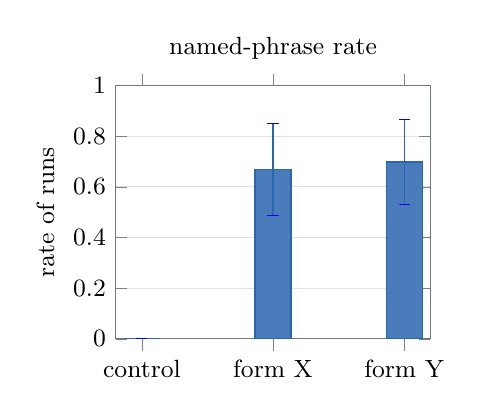
\begin{tikzpicture}
\begin{axis}[width=0.46\textwidth,height=4.8cm,ybar,bar width=13pt,
  ymin=0,ymax=1.0,ylabel={rate of runs},title={\small named-phrase rate},
  symbolic x coords={control,form X,form Y},xtick=data,
  axis line style={inkmut},tick label style={font=\small},
  ylabel style={font=\small},ymajorgrids,grid style={inkmut!22},
  error bars/y dir=both,error bars/y explicit]
\addplot+[fill=accent!85,draw=accent] coordinates {
  (control,0.000) +- (0,0)
  (form X,0.667) +- (0.207,0.182)
  (form Y,0.698) +- (0.174,0.167)};
\end{axis}
\end{tikzpicture}\hfill
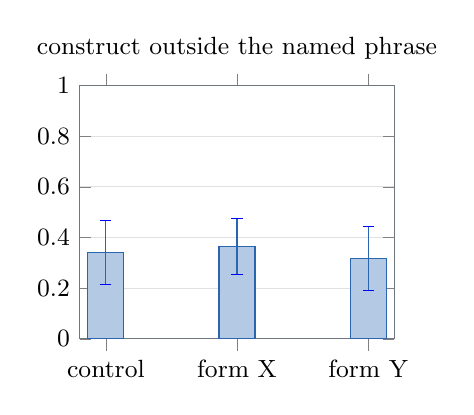
\begin{tikzpicture}
\begin{axis}[width=0.46\textwidth,height=4.8cm,ybar,bar width=13pt,
  ymin=0,ymax=1.0,title={\small construct outside the named phrase},
  symbolic x coords={control,form X,form Y},xtick=data,
  axis line style={inkmut},tick label style={font=\small},
  ymajorgrids,grid style={inkmut!22},
  error bars/y dir=both,error bars/y explicit]
\addplot+[fill=accent!35,draw=accent] coordinates {
  (control,0.341) +- (0.119,0.127)
  (form X,0.365) +- (0.111,0.111)
  (form Y,0.317) +- (0.119,0.127)};
\end{axis}
\end{tikzpicture}
\caption{The phrase-swap experiment (378 runs, cluster-bootstrap 95\%
CIs over 18 cases). \textbf{Left}: each instructed arm produces its own
named phrase in about two thirds of runs; control never produces
either, and cross-form leakage is $0/252$. \textbf{Right}: the
validated-judge construct rate outside the named phrase is
statistically indistinguishable across all three arms. The
instruction's entire measurable effect is the phrase it names.}
\label{fig:swap}
\end{figure*}

The recipe's aggregate-and-synthesize prompt asks the aggregator to be
critical, preserve accuracy, and weigh its sources. Whether such
instructions change behavior or only wording was tested by
Equation~\ref{eq:entangle}'s required design. Three arms were run on 18
cases with 7 repeats (378 runs): a minimal writer prompt as control,
and two treated arms appending a byte-identical clause differing in
exactly three words, instructing the writer to label estimates with
the phrase ``modeled at'' (form X) or ``taken to be'' (form Y). Form X
had been dictated through months of the program's prompts; form Y was
chosen the day before the run and appears nowhere in 2M characters of
archive. Each instructed arm produced its own phrase in about two
thirds of outputs ($0.667$, $0.698$); control produced neither;
cross-form leakage was $0/252$ (Figure~\ref{fig:swap}, left). With each
arm's own phrase subtracted, the validated-judge construct rate was
unchanged: form X moved from $0.341$ to $0.365$ (\ci{-0.079}{+0.111}),
form Y from $0.341$ to $0.317$ (\ci{-0.103}{+0.087}), with emission
flat across arms (Figure~\ref{fig:swap}, right). The registered
minimum detectable effect was $+0.224$, so the result licenses ``no
form-independent effect of at least $0.22$'' rather than zero. A
months-old house phrase and a day-old synonym performed identically:
whatever the instruction engages, it is not a learned disposition.

\subsection{Preference Rewards Aggregation and Penalizes the Phrase}
\label{sec:pref}

\begin{figure}[t]
\centering
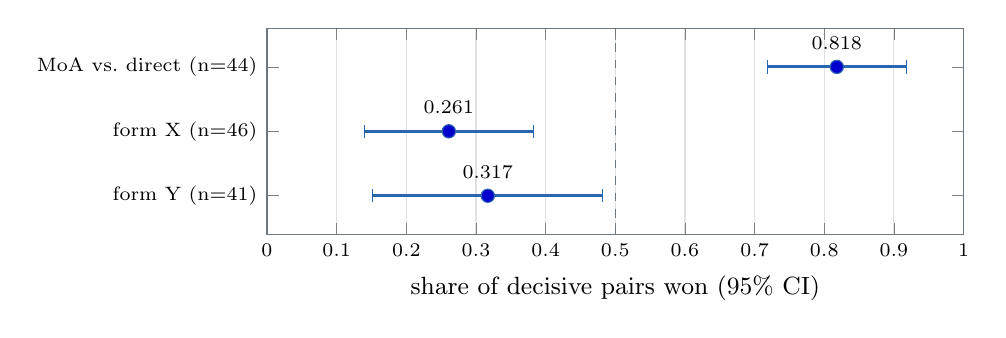
\begin{tikzpicture}
\begin{axis}[width=0.86\columnwidth,height=4.2cm,xmin=0,xmax=1,
  ytick={1,2,3},yticklabels={form Y (n=41),
  form X (n=46), MoA vs.\ direct (n=44)},
  ymin=0.4,ymax=3.6,xlabel={share of decisive pairs won (95\% CI)},
  tick label style={font=\scriptsize},xlabel style={font=\small},
  axis line style={inkmut},xmajorgrids,grid style={inkmut!22}]
\addplot+[only marks,mark=*,mark size=2.4pt,color=accent,
  error bars/.cd,x dir=both,x explicit,error bar style={line width=1pt}]
  coordinates {
  (0.818,3) +- (0.100,0.101)
  (0.261,2) +- (0.121,0.127)
  (0.317,1) +- (0.165,0.163)};
\addplot[dashed,inkmut] coordinates {(0.5,0.4) (0.5,3.6)};
\node[font=\scriptsize,anchor=south] at (axis cs:0.818,3.12) {0.818};
\node[font=\scriptsize,anchor=south] at (axis cs:0.261,2.12) {0.261};
\node[font=\scriptsize,anchor=south] at (axis cs:0.317,1.12) {0.317};
\end{axis}
\end{tikzpicture}
\caption{The preference experiment under Equation~\ref{eq:pref}. The
aggregated pipeline beats the matched-length direct baseline; both
phrase-instructed arms lose to their own control, in counterbalanced
forms whose only difference from control is the phrase. The dashed
line is indifference.}
\label{fig:pref}
\end{figure}

Three pairwise comparisons were run on the same 18 cases (126 pairs
each; both orderings; primary judge \texttt{gpt-oss:20b}, which also
wrote both sides of every pair, making self-preference symmetric). The
aggregated pipeline beat the same writer answering directly in $0.818$
\ci{0.718}{0.919} of 44 decisive pairs. Arm lengths differed by
$1.4\%$, the share among near-length-matched pairs was $0.815$, and the
winner had more domain frameworks per kilocharacter in only $0.409$ of
decisive pairs, so the lift is neither length nor framework density;
its composition is unidentified by the available feature set. The
phrase-instructed arms, which differ from control only in the phrase,
lost to control at $0.261$ \ci{0.140}{0.388} (form X) and $0.317$
\ci{0.152}{0.480} (form Y), against a registered prediction of the
opposite (Figure~\ref{fig:pref}). A second judge from a disjoint
family (a 30B Qwen3 MoE, selected blind to direction) replicated the
lift ($0.788$ \ci{0.645}{0.917}) and the form-Y penalty ($0.217$
\ci{0.125}{0.333}); the form-X penalty agreed in point estimate
($0.276$) with an interval spanning $0.5$ at $n{=}29$ and is reported
as not replicated at that power. Chained with
Section~\ref{sec:phrase}, both links causal: an epistemic instruction
installs only a surface form, and a preference judge penalizes that
form. A pipeline tuned toward judge preference will shed exactly the
marking that instructions install while the underlying disposition,
untouched by the instruction, stays where it was.

\subsection{The Aggregator Selects Sources and Never Verifies}
\label{sec:select}

\begin{figure}[t]
\centering
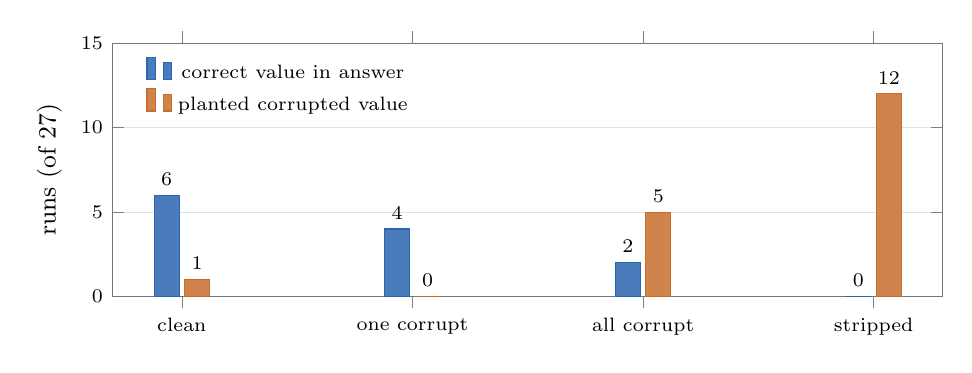
\begin{tikzpicture}
\begin{axis}[width=\columnwidth,height=4.8cm,ybar,bar width=9pt,
  ymin=0,ymax=15,ylabel={runs (of 27)},
  symbolic x coords={clean,one corrupt,all corrupt,stripped},xtick=data,
  axis line style={inkmut},tick label style={font=\scriptsize},
  ylabel style={font=\small},ymajorgrids,grid style={inkmut!22},
  legend style={font=\scriptsize,draw=none,at={(0.03,0.97)},anchor=north west},
  nodes near coords,nodes near coords style={font=\scriptsize,text=black}]
\addplot+[fill=accent!85,draw=accent] coordinates {
  (clean,6) (one corrupt,4) (all corrupt,2) (stripped,0)};
\addplot+[fill=corrupt!85,draw=corrupt] coordinates {
  (clean,1) (one corrupt,0) (all corrupt,5) (stripped,12)};
\legend{correct value in answer,planted corrupted value}
\end{axis}
\end{tikzpicture}
\caption{The source-selector gradient (planted arithmetic errors; exact
match on known values). As clean sources are removed, adoption of the
planted wrong value rises monotonically through $1$, $0$, $5$, and $12$
runs while correct values vanish.}
\label{fig:grad}
\end{figure}

With arithmetic claims planted in proposer texts, a corrupted value
reached the answer $0/27$ times when one proposer was corrupted and a
clean one remained, $5/27$ when every proposer was corrupted, and
$12/27$ when the working was also stripped (Figure~\ref{fig:grad}). A
later single-factor experiment sharpened the bare case: a sole-sourced
corrupted value is adopted at $0.900$. The aggregator prefers
uncorrupted sources when they exist and has no independent hold on the
content when they do not. MoA's observation that the aggregator's
output overlaps most with the best proposals \cite{wang2024moa} is the
same phenomenon from the benign side; the planted-error view adds the
failure boundary, and the claim of improvement even from worse inputs
fails at the fact level.

\subsection{Corroboration Is Ignored and Transport Is Weak}
\label{sec:transport}

Claims advanced by two or more independent proposers transport to the
final answer no more often than single-proposer claims ($0.487$
against $0.524$; difference CI \ci{-0.153}{+0.080}). Epistemic
qualification fares worse. Across 144 runs, two writers, and two
corpora, the within-corpus slope $w$ of Equation~\ref{eq:transport}
runs from $0.105$ to $0.326$, three of four fits excluding zero, with
the extension-corpus fit replicating on nine cases the original corpus
never contained (Figure~\ref{fig:transport}). The writer emits roughly
one sixth to one third of the caution it is given, the fraction is a
property of the writing step rather than of one model, and the writer
also invents qualification at $0.333$ \ci{0.138}{0.609} on inputs
confirmed to contain none.

\begin{figure*}[t]
\centering
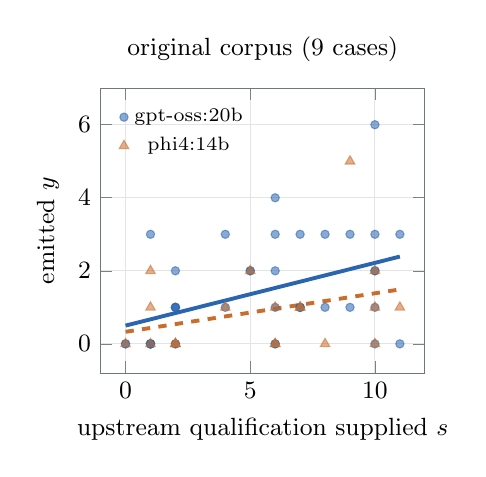
\begin{tikzpicture}
\begin{axis}[width=0.47\textwidth,height=5.2cm,
  xmin=-1,xmax=12,ymin=-0.8,ymax=7,
  xlabel={upstream qualification supplied $s$},ylabel={emitted $y$},
  title={\small original corpus (9 cases)},
  axis line style={inkmut},tick label style={font=\small},
  xlabel style={font=\small},ylabel style={font=\small},
  ymajorgrids,xmajorgrids,grid style={inkmut!20},legend style={font=\scriptsize,draw=none,at={(0.03,0.97)},anchor=north west,fill=none},]
\addplot[only marks,mark=*,mark size=1.5pt,color=accent,opacity=0.55]
  coordinates {(1.0,0.0) (1.0,0.0) (1.0,3.0) (1.0,0.0) (8.0,1.0) (8.0,3.0) (10.0,1.0) (10.0,0.0) (10.0,3.0) (10.0,2.0) (11.0,3.0) (11.0,0.0) (6.0,3.0) (6.0,1.0) (7.0,3.0) (7.0,1.0) (5.0,2.0) (5.0,2.0) (6.0,2.0) (6.0,0.0) (4.0,1.0) (4.0,3.0) (2.0,1.0) (2.0,2.0) (6.0,0.0) (6.0,4.0) (7.0,1.0) (7.0,1.0) (2.0,1.0) (2.0,1.0) (9.0,1.0) (9.0,3.0) (10.0,6.0) (10.0,2.0) (0.0,0.0) (0.0,0.0) (2.0,0.0) (2.0,0.0) (1.0,0.0) (1.0,0.0)};
\addplot[only marks,mark=triangle*,mark size=2pt,color=corrupt,opacity=0.55]
  coordinates {(1.0,1.0) (1.0,2.0) (8.0,0.0) (10.0,1.0) (10.0,2.0) (11.0,1.0) (6.0,0.0) (7.0,1.0) (5.0,2.0) (6.0,1.0) (4.0,1.0) (2.0,0.0) (6.0,0.0) (7.0,1.0) (2.0,0.0) (9.0,5.0) (10.0,0.0) (0.0,0.0) (2.0,0.0) (1.0,0.0)};
\addplot[accent,line width=1.4pt] coordinates {(0.0,0.50) (11.0,2.39)};
\addplot[corrupt,line width=1.4pt,dashed] coordinates {(0.0,0.33) (11.0,1.49)};
\legend{gpt-oss:20b,phi4:14b}
\end{axis}
\end{tikzpicture}\hfill
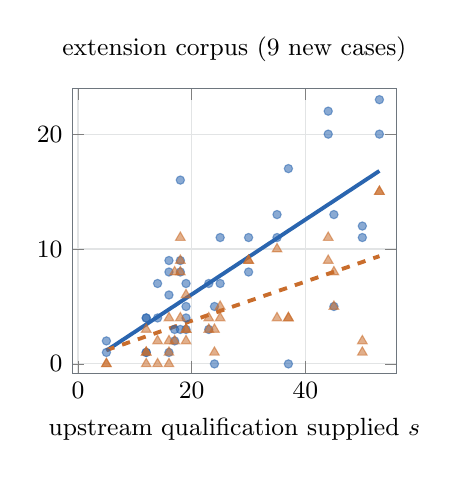
\begin{tikzpicture}
\begin{axis}[width=0.47\textwidth,height=5.2cm,
  xmin=-1,xmax=56,ymin=-0.8,ymax=24,
  xlabel={upstream qualification supplied $s$},
  title={\small extension corpus (9 new cases)},
  axis line style={inkmut},tick label style={font=\small},
  xlabel style={font=\small},ylabel style={font=\small},
  ymajorgrids,xmajorgrids,grid style={inkmut!20},]
\addplot[only marks,mark=*,mark size=1.5pt,color=accent,opacity=0.55]
  coordinates {(5,1) (5,2) (12,4) (12,4) (12,1) (12,1) (18,9) (18,8) (18,16) (18,3) (19,7) (19,4) (23,3) (23,7) (44,22) (44,20) (53,20) (53,23) (16,8) (16,9) (16,6) (16,1) (14,4) (14,7) (24,0) (24,5) (19,3) (19,5) (17,2) (17,3) (25,11) (25,7) (37,17) (37,0) (50,11) (50,12) (30,11) (30,8) (35,11) (35,13) (45,5) (45,13)};
\addplot[only marks,mark=triangle*,mark size=2pt,color=corrupt,opacity=0.55]
  coordinates {(5,0) (5,0) (12,3) (12,0) (12,1) (12,1) (18,11) (18,8) (18,9) (18,4) (19,3) (19,6) (23,4) (23,3) (44,11) (44,9) (53,15) (53,15) (16,0) (16,2) (16,1) (16,4) (14,0) (14,2) (24,1) (24,3) (19,2) (19,3) (17,8) (17,2) (25,5) (25,4) (37,4) (37,4) (50,2) (50,1) (30,9) (30,9) (35,4) (35,10) (45,5) (45,8)};
\addplot[accent,line width=1.4pt] coordinates {(5,1.16) (53,16.80)};
\addplot[corrupt,line width=1.4pt,dashed] coordinates {(5,1.20) (53,9.38)};
\end{axis}
\end{tikzpicture}
\caption{The transport coefficient of Equation~\ref{eq:transport}, 144
runs over 18 cases and two writers; each point is one run, both
quantities counted by the validated two-judge sentence protocol, lines
are within-panel least-squares fits. Within-panel slopes:
\mbox{gpt-oss} $0.172$ \ci{+0.052}{+0.297} and $0.326$
\ci{+0.207}{+0.434}; phi4 $0.105$ \ci{-0.031}{+0.273} and $0.170$
\ci{+0.067}{+0.265}. Panels are separated because the corpora occupy
different supply regimes (mean $s$ of $5.4$ against $25.3$).}
\label{fig:transport}
\end{figure*}

\subsection{Specialists Carry Per-Model Signatures}
\label{sec:signature}

Two medical fine-tunes of the same base model do not share a domain
signature: one shifts in-domain framework density $+0.232$
\ci{+0.072}{+0.412} over the base, the other $+0.109$
\ci{-0.056}{+0.300}, and a second lineage shows $-0.041$
\ci{-0.099}{+0.025}. A descriptive check found two same-domain seats
no more distant from each other than one seat is from itself across
samples, consistent with the Self-MoA result \cite{li2025selfmoa} at
benchmark scale. Seating a model for its domain label has no measured
warrant.

\subsection{Self-Assessment Predicts Behavior at Chance}
\label{sec:selfassess}

Seats given a roster and a structured deferral token route to the
correct colleague when they defer ($10/11$, $0.909$
\ci{0.623}{0.984}) but defer about as often in-domain as out-of-domain
($0.083$ against $0.306$; difference CI \ci{-0.056}{+0.528}). A model's
own plausibility rating predicted which planted values it would adopt
at $0.544$. A stable, near-unanimous elicited map of which seat owns
each quantity predicted arbitration on fresh items at exactly $0.500$
against a descriptive $0.895$. In every consultation design measured,
the mechanism worked when fired and the firing was rare: the lead used
a routed clarification in $7/7$ runs but named the tension warranting
it at $0.34$, and across three experiments the trigger rate ranged
from $0.208$ to $0.583$ by batch. Self-assessment, the faculty that
escalation designs rely on, was the one faculty the program never
found.

\subsection{Accuracy Is Untestable at This Scale}
\label{sec:accuracy}

On a 60-item self-verifying battery the aggregated pipeline and the
bare writer were indistinguishable at a $0.92$ to $0.97$ ceiling. Two
registered follow-up batteries (36 multi-step computation items and 30
rule-interaction items with script-computed answers, under
baseline-only difficulty screens) placed the direct writer at $0.977$
and $0.983$. Under the pre-registered two-strikes rule the question is
resolved as untestable for lack of headroom. The harness claims no
accuracy gain and is not designed to produce one.

\begin{table}[t]
\centering\small
\setlength{\tabcolsep}{4pt}
\begin{tabular}{p{0.36\columnwidth}p{0.20\columnwidth}p{0.34\columnwidth}}
\toprule
Failure of the recipe & Measurement & Mechanism licensed \\
\midrule
Instructions install only their phrase (\S\ref{sec:phrase}) & construct unchanged, MDE $0.22$ & no disposition instructions to the lead \\
Judges penalize the phrase (\S\ref{sec:pref}) & $0.261$, $0.317$ vs.\ control & out-of-band channel; charter \\
Aggregator selects, never verifies (\S\ref{sec:select}) & $0.900$ sole-sourced; $0/27$ with co-source & engineered redundancy \\
Corroboration ignored; transport weak (\S\ref{sec:transport}) & $w = 0.11$ to $0.33$ & out-of-band channel \\
Per-model signatures (\S\ref{sec:signature}) & $+0.232$, $+0.109$, $-0.041$ & empirical seating gate \\
Self-assessment at chance (\S\ref{sec:selfassess}) & $0.544$; $0.500$ & artifact-triggered re-consultation \\
Accuracy at ceiling (\S\ref{sec:accuracy}) & $0.92$ to $0.98$ direct & no accuracy claim \\
\bottomrule
\end{tabular}
\caption{Each failure mode of the recipe, its measurement, and the
harness mechanism it licenses.}
\label{tab:map}
\end{table}

\section{Evidence-Bound Harness}
\label{sec:harness}

The harness retains the recipe's structure and preference lift and
adds the five mechanisms of Table~\ref{tab:map}.
Figure~\ref{fig:arch} shows the assembled pipeline with every edge
labeled by its registered measurement.

\begin{figure*}[t]
\centering
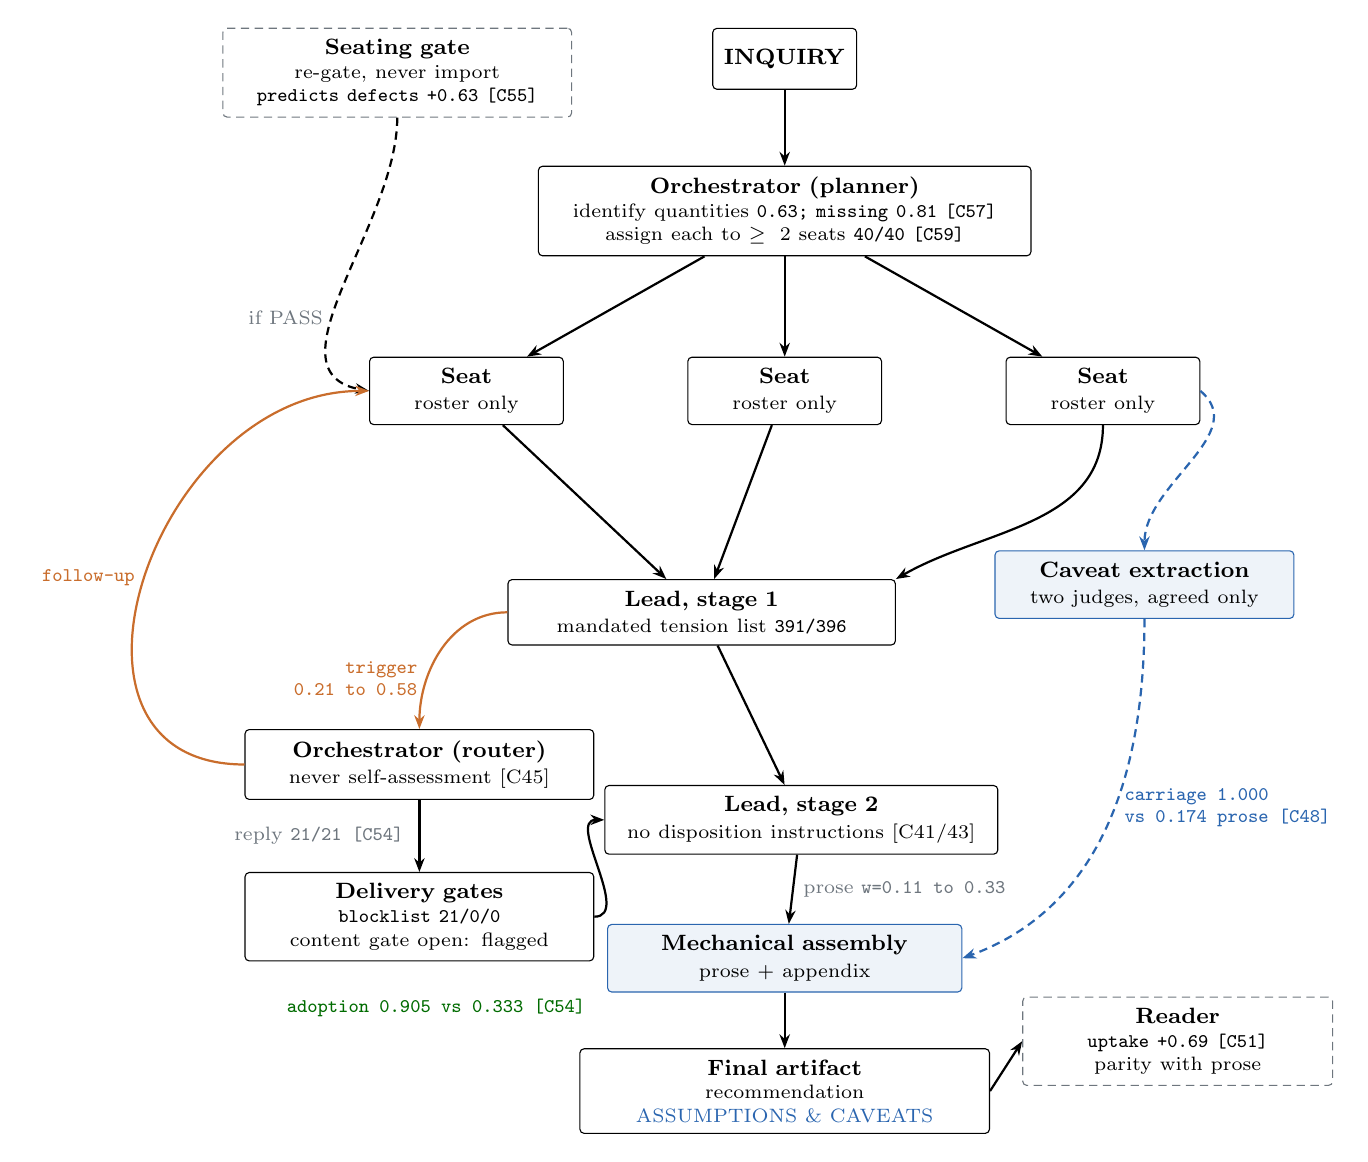
\begin{tikzpicture}[x=1pt,y=1pt,font=\footnotesize,
  box/.style={draw,rounded corners=1.5pt,align=center,inner sep=4pt,minimum height=22pt},
  gate/.style={box,densely dashed,draw=inkmut},
  frt/.style={box,draw=accent,fill=accent!8},
  ed/.style={-{Stealth[length=5pt]},thick},
  edf/.style={-{Stealth[length=5pt]},thick,accent,densely dashed},
  edl/.style={-{Stealth[length=5pt]},thick,corrupt},
  n/.style={font=\scriptsize\ttfamily,text=accent},
  ng/.style={font=\scriptsize\ttfamily,text=black!30!green!60!black},
  nr/.style={font=\scriptsize\ttfamily,text=corrupt},
  s/.style={font=\scriptsize,text=inkmut}]
\node[box] (q) at (170,395) {\textbf{INQUIRY}};
\node[gate,text width=118pt] (sg) at (30,390)
  {\textbf{Seating gate}\\[-1pt]{\scriptsize re-gate, never import}\\[-1pt]
   {\scriptsize\ttfamily predicts defects +0.63 [C55]}};
\node[box,text width=170pt] (pl) at (170,340)
  {\textbf{Orchestrator (planner)}\\[-1pt]
   {\scriptsize identify quantities \ttfamily 0.63; missing 0.81 [C57]}\\[-1pt]
   {\scriptsize assign each to $\ge2$ seats \ttfamily 40/40 [C59]}};
\node[box,text width=62pt] (s1) at (55,275) {\textbf{Seat}\\{\scriptsize roster only}};
\node[box,text width=62pt] (s2) at (170,275) {\textbf{Seat}\\{\scriptsize roster only}};
\node[box,text width=62pt] (s3) at (285,275) {\textbf{Seat}\\{\scriptsize roster only}};
\node[frt,text width=100pt] (cv) at (300,205)
  {\textbf{Caveat extraction}\\{\scriptsize two judges, agreed only}};
\node[box,text width=132pt] (l1) at (140,195)
  {\textbf{Lead, stage 1}\\{\scriptsize mandated tension list \ttfamily 391/396}};
\node[box,text width=118pt] (rt) at (38,140)
  {\textbf{Orchestrator (router)}\\{\scriptsize never self-assessment [C45]}};
\node[box,text width=118pt] (gt) at (38,85)
  {\textbf{Delivery gates}\\[-1pt]
   {\scriptsize\ttfamily blocklist 21/0/0}\\[-1pt]
   {\scriptsize content gate open: flagged}};
\node[box,text width=134pt] (l2) at (176,120)
  {\textbf{Lead, stage 2}\\{\scriptsize no disposition instructions [C41/43]}};
\node[frt,text width=120pt] (asm) at (170,70)
  {\textbf{Mechanical assembly}\\{\scriptsize prose + appendix}};
\node[box,text width=140pt] (fin) at (170,22)
  {\textbf{Final artifact}\\[-1pt]{\scriptsize recommendation}\\[-1pt]
   {\color{accent}\scriptsize ASSUMPTIONS \& CAVEATS}};
\node[gate,text width=104pt] (rd) at (312,40)
  {\textbf{Reader}\\[-1pt]{\scriptsize\ttfamily uptake +0.69 [C51]}\\[-1pt]
   {\scriptsize parity with prose}};
\draw[ed] (q) -- (pl);
\draw[ed,densely dashed] (sg.south) to[out=-90,in=170] node[s,left,pos=.6]{if PASS} (s1.west);
\draw[ed] (pl) -- (s1); \draw[ed] (pl) -- (s2); \draw[ed] (pl) -- (s3);
\draw[ed] (s1) -- (l1); \draw[ed] (s2) -- (l1);
\draw[ed] (s3.south) to[out=-90,in=30] (l1.north east);
\draw[edf] (s3.east) to[out=-40,in=90] (cv.north);
\draw[edf] (cv.south) to[out=-90,in=20]
  node[n,right,pos=.45,align=left]{carriage 1.000\\vs 0.174 prose [C48]} (asm.east);
\draw[edl] (l1.west) to[out=180,in=90]
  node[nr,left,pos=.7,align=right]{trigger\\0.21 to 0.58} (rt.north);
\draw[edl] (rt.west) to[out=180,in=180,looseness=1.4]
  node[nr,left,pos=.5,align=right]{follow-up} (s1.west);
\draw[ed] (rt) -- node[s,left=2pt]{reply \ttfamily 21/21 [C54]} (gt);
\draw[ed] (gt.east) to[out=0,in=180] (l2.west);
\node[ng] at (44,52) {adoption 0.905 vs 0.333 [C54]};
\draw[ed] (l1) -- (l2);
\draw[ed] (l2) -- node[s,right]{prose \ttfamily w=0.11 to 0.33} (asm);
\draw[ed] (asm) -- (fin);
\draw[ed] (fin.east) -- (rd.west);
\end{tikzpicture}
\caption{The harness on one inquiry, with every edge labeled by its
registered measurement (bracketed codes are ledger entries). Dashed
blue: the out-of-band channel for epistemic qualification, which the
writer never sees. Orange: the orchestrator-routed re-consultation
loop, bounded by its measured trigger rate. Chairs are earned by the
gate, never by category label, and engineered overlap between seats is
where error immunity resides.}
\label{fig:arch}
\end{figure*}

\subsection{Empirical Seating Gate}

Because signatures are per-model (Section~\ref{sec:signature}), no
seat is chaired for its category label. A candidate passes a frozen
gate consisting of a degeneracy screen (at least $800$ visible
characters on screen items; one archive fine-tune produced $12/12$
degenerate probe runs), a tuned-minus-own-base signature probe, and a
format smoke test at production token budgets. A generalist under a
role prompt is a legitimate seat if it passes. Verdicts are
re-computed at seating time, never imported from the archive
(Section~\ref{sec:res-gate}).

\subsection{Isolation on Cost Grounds}

Seats receive a self-contained sub-question and a one-line roster;
sibling outputs are not forwarded. The rule was adopted on a
contamination rationale that a registered test later withdrew
(Section~\ref{sec:ablations}); it stands because sibling context costs
approximately $10$k input characters and $14\%$ longer outputs per
seat while purchasing no measured change in lane discipline.

\subsection{Engineered Redundancy}

Because the lead selects among sources and never verifies
(Section~\ref{sec:select}), protection is coverage. The planner
identifies the load-bearing quantities in the decomposition and
writes each into the sub-questions of at least two seats. Expected
protection is the product of identification coverage and the
selection effect,
\begin{equation}
\begin{aligned}
\Pr[\text{clean adopted}] \approx{} & \Pr[\text{identified}] \\
& \times \Pr[\text{clean selected} \mid \text{covered}],
\end{aligned}
\label{eq:protection}
\end{equation}
and is stated as expected value only (Section~\ref{sec:res-planner}).

\subsection{Artifact-Triggered Re-consultation}

Because self-assessment predicts behavior at chance
(Section~\ref{sec:selfassess}), no model decides whether it needs
help. The lead runs in two stages: a mandated tension list first
($391/396$ archived runs produce one when required), then synthesis.
The orchestrator parses the list and dispatches a follow-up
sub-question to the implicated seat. Replies pass through a
fabrication blocklist seeded from committed classifications and a
content flag for replies adding nothing beyond the seat's first
contribution; flagged replies are delivered with the flag rather than
dropped, because the content gate did not meet its frozen criteria
(Section~\ref{sec:ablations}).

\subsection{Out-of-Band Epistemic Channel}

Because prose transports a small fraction of supplied qualification
(Section~\ref{sec:transport}) and preference judges penalize the
visible marking that instructions install (Section~\ref{sec:pref}),
caveats, assumptions, and confidence never route through the writer.
Seats emit them as structured fields; a two-judge extraction retains
only sentences both judges agree carry qualification; and the harness
assembles them mechanically into an appendix of the final artifact.
The writer receives no disposition instructions at all.

\subsection{Goodhart Charter}

Trigger rates, hedge counts, compliance shares, transport slopes, and
preference scores on epistemic content are diagnostics and may never
be optimization targets; the optimizable signal must live outside the
pipeline's own text. Each forbidden entry cites the experiment that
showed what optimizing it would manufacture (Appendix~\ref{app:charter}).

\section{Experimental Setup}
\label{sec:setup}

\textbf{Pipeline and cases.} The auditable instance is a two-layer MoA:
three proposer seats (prompted or domain-fine-tuned 7 to 8B models, or
role-prompted samples of the writer) whose contributions are
concatenated for a 20B mixture-of-experts writer
(\texttt{gpt-oss:20b}). A lead planner performs step-back
decomposition and dispatches a self-contained sub-question to each
seat. The case battery is eighteen strategic advisory scenarios
spanning healthcare, legal, and finance content; individual
experiments use subsets of 6 to 18 cases, and every confidence
interval is a cluster bootstrap over cases.

\textbf{Registration.} Every experiment is registered before it runs
with its hypotheses, falsification conditions, attainability
computation (the fraction of runs in which the outcome variable can
fire, computed from existing data), and consequences. Verdicts enter a
ledger distinguishing live, provisional, withdrawn, and blocked
claims; three program-level audits re-classified earlier results, and
nulls are cited only at the strength their audit class permits.
Registrations are committed before first runs, so temporal ordering
is verifiable from version history.

\textbf{Instruments.} Construct presence is scored by a two-judge,
batched, sentence-level protocol whose definitions name no phrase;
agreement on the deployed corpus is $0.910$ (14{,}088/15{,}485
decisions). A frozen dictation registry of every phrase any prompt
places in a model's mouth (125 entries) gates all prompts, with a
measured over-attribution of zero across 2{,}907 clean-provenance
spans. Preference is judged in both orders with agreement required
(Equation~\ref{eq:pref}); raw first-position preference is $0.85$ to
$0.88$ across four judge families, and debiasing converts $60$ to
$95\%$ of pairs to ties (Appendix~\ref{app:instruments}).

\textbf{Baselines.} The unmodified pipeline (the recipe as published,
with the MoA aggregate-and-synthesize prompt or a minimal lead
prompt), the direct writer (same model, same cases, prompt minus the
sentence referencing contributions), and, for re-consultation, a
scripted-reply ceiling and a length-matched contentless-reply control.

\textbf{Metrics.} Corrupted and clean \emph{adoption} (exact match on
planted values); \emph{carriage} (share of both-judge caveat sentences
reaching the final artifact); \emph{uptake} (share of a reader model's
registered two-token decisions flipped by a delivered caveat, with
direction-balanced items); \emph{defect rate} (share of a seat's
contributions violating its lane); \emph{trigger rate}; and the
order-debiased \emph{preference share} of Equation~\ref{eq:pref}.

\section{Results}
\label{sec:results}

Each mechanism received its own registered single-factor experiment
with kill conditions stated in advance. Table~\ref{tab:main} collects
the main results against the unmodified pipeline and
Figure~\ref{fig:prepost} plots them; the subsections give the
measurements.

\begin{figure*}[t]
\centering
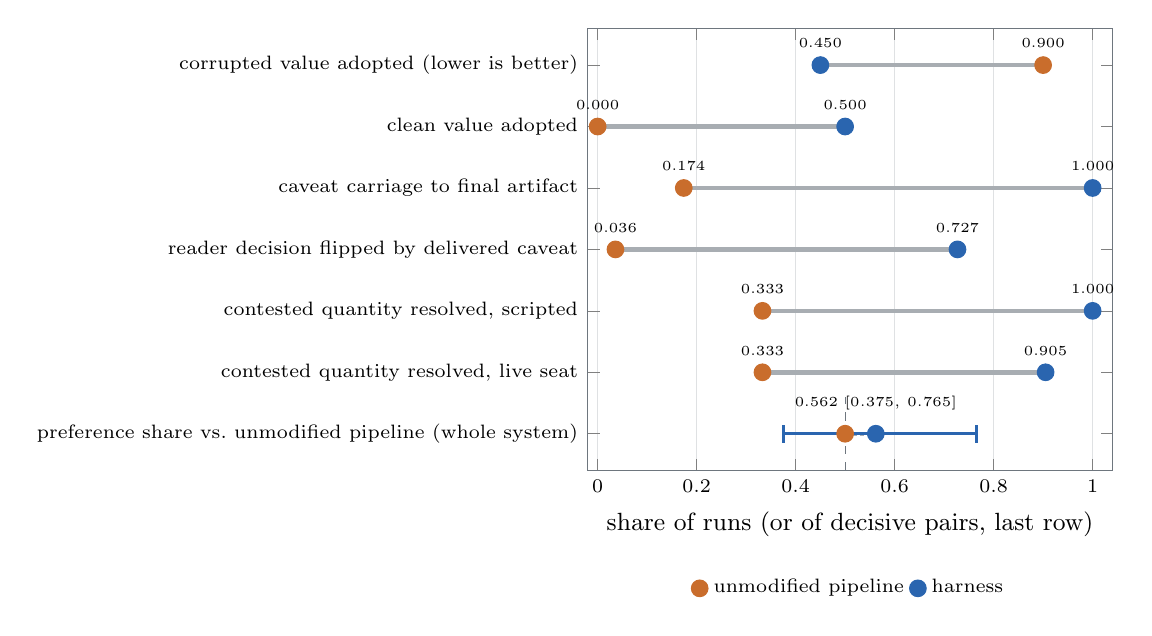
\begin{tikzpicture}
\begin{axis}[width=0.68\textwidth,height=7.2cm,
  xmin=-0.02,xmax=1.04,ymin=0.4,ymax=7.6,
  xlabel={share of runs (or of decisive pairs, last row)},
  ytick={1,...,7},
  yticklabels={
    {preference share vs.\ unmodified pipeline (whole system)},
    {contested quantity resolved, live seat},
    {contested quantity resolved, scripted},
    {reader decision flipped by delivered caveat},
    {caveat carriage to final artifact},
    {clean value adopted},
    {corrupted value adopted (lower is better)}},
  yticklabel style={font=\scriptsize,align=right},
  tick label style={font=\scriptsize},xlabel style={font=\small},
  axis line style={inkmut},xmajorgrids,grid style={inkmut!22},
  legend style={font=\scriptsize,draw=none,at={(0.5,-0.22)},anchor=north,fill=none},
  legend columns=2,legend cell align=left,clip=false]
% connectors
\draw[inkmut!60,line width=1.6pt] (axis cs:0.900,7) -- (axis cs:0.450,7);
\draw[inkmut!60,line width=1.6pt] (axis cs:0.000,6) -- (axis cs:0.500,6);
\draw[inkmut!60,line width=1.6pt] (axis cs:0.174,5) -- (axis cs:1.000,5);
\draw[inkmut!60,line width=1.6pt] (axis cs:0.036,4) -- (axis cs:0.727,4);
\draw[inkmut!60,line width=1.6pt] (axis cs:0.333,3) -- (axis cs:1.000,3);
\draw[inkmut!60,line width=1.6pt] (axis cs:0.333,2) -- (axis cs:0.905,2);
\draw[inkmut!60,line width=1.6pt,densely dotted] (axis cs:0.500,1) -- (axis cs:0.562,1);
% CI on the head-to-head row
\draw[accent,line width=1pt] (axis cs:0.375,1) -- (axis cs:0.765,1);
\draw[accent,line width=1pt] (axis cs:0.375,0.85) -- (axis cs:0.375,1.15);
\draw[accent,line width=1pt] (axis cs:0.765,0.85) -- (axis cs:0.765,1.15);
\addplot[only marks,mark=*,mark size=3pt,color=corrupt,mark options={fill=corrupt}]
  coordinates {(0.900,7) (0.000,6) (0.174,5) (0.036,4) (0.333,3) (0.333,2) (0.500,1)};
\addlegendentry{unmodified pipeline}
\addplot[only marks,mark=*,mark size=3pt,color=accent,mark options={fill=accent}]
  coordinates {(0.450,7) (0.500,6) (1.000,5) (0.727,4) (1.000,3) (0.905,2) (0.562,1)};
\addlegendentry{harness}
\addplot[dashed,inkmut] coordinates {(0.5,0.4) (0.5,1.6)};
% direct labels
\node[font=\tiny,anchor=south] at (axis cs:0.900,7.12) {0.900};
\node[font=\tiny,anchor=south] at (axis cs:0.450,7.12) {0.450};
\node[font=\tiny,anchor=south] at (axis cs:0.000,6.12) {0.000};
\node[font=\tiny,anchor=south] at (axis cs:0.500,6.12) {0.500};
\node[font=\tiny,anchor=south] at (axis cs:0.174,5.12) {0.174};
\node[font=\tiny,anchor=south] at (axis cs:1.000,5.12) {1.000};
\node[font=\tiny,anchor=south] at (axis cs:0.036,4.12) {0.036};
\node[font=\tiny,anchor=south] at (axis cs:0.727,4.12) {0.727};
\node[font=\tiny,anchor=south] at (axis cs:0.333,3.12) {0.333};
\node[font=\tiny,anchor=south] at (axis cs:1.000,3.12) {1.000};
\node[font=\tiny,anchor=south] at (axis cs:0.333,2.12) {0.333};
\node[font=\tiny,anchor=south] at (axis cs:0.905,2.12) {0.905};
\node[font=\tiny,anchor=south] at (axis cs:0.562,1.22) {0.562 \ci{0.375}{0.765}};
\end{axis}
\end{tikzpicture}
\caption{Outcomes before and after the harness. Each of the first six
rows is one registered single-factor experiment in which the
unmodified pipeline (orange) and the harness mechanism (blue) were
measured on the same outcome; the rows are separate experiments, not
one before-and-after run of the whole system. The last row is the only
whole-system comparison, the order-debiased head-to-head of
Section~\ref{sec:headtohead}, with its 95\% interval spanning the
dashed indifference line. Corrupted-value adoption is the one row where
lower is better. Values and intervals are those of Table~\ref{tab:main}.}
\label{fig:prepost}
\end{figure*}

\begin{table*}[t]
\centering\footnotesize
\setlength{\tabcolsep}{4pt}
\resizebox{\textwidth}{!}{%
\begin{tabular}{p{0.30\textwidth}lccl}
\toprule
Outcome & Mechanism under test & Unmodified pipeline & Harness & Verdict \\
\midrule
Corrupted value adopted (sole-sourced) $\downarrow$ & engineered redundancy & $0.900$ & \bestcell $0.450$ \ci{+0.200}{+0.725} & survived (causal) \\
Clean value adopted $\uparrow$ & engineered redundancy & $0.000$ & \bestcell $0.500$ \ci{+0.175}{+0.825} & survived \\
Clean co-source used end-to-end $\uparrow$ & planner, live & planted $+0.500$ & \bestcell $+0.425$ \ci{+0.325}{+0.525} & survived \\
Caveat carriage to artifact $\uparrow$ & out-of-band channel & $0.174$ & \bestcell $1.000$ & survived \\
Reader decision flipped by caveat $\uparrow$ & out-of-band channel & $0.036$ (irrelevant ctrl.) & \bestcell $0.727$ & survived \\
Contested quantity resolved (scripted) $\uparrow$ & re-consultation & $0.333$ & \bestcell $1.000$ ($7/7$) & survived \\
Contested quantity resolved (live seat) $\uparrow$ & re-consultation & $0.333$ & \bestcell $0.905$ & survived, one halt \\
Seat defect rate, gate-pass vs.\ gate-fail $\downarrow$ & seating gate & $0.333$, $0.944$ (fail) & \bestcell $0.000$ to $0.056$ (pass) & survived \\
Preference share vs.\ unmodified pipeline & assembled harness & $0.500$ (reference) & $0.562$ \ci{0.375}{0.765} & no evaluable difference \\
\bottomrule
\end{tabular}}
\caption{Main results. Each row is one registered single-factor
experiment; shaded cells mark the harness where its interval excludes
the baseline. The final row is the head-to-head of
Section~\ref{sec:headtohead}, in which no difference is evaluable and
no cell is shaded.}
\label{tab:main}
\end{table*}

\subsection{Seating Gate}
\label{sec:res-gate}

Ten local candidates were gated on the frozen degeneracy screen using
two screen items disjoint from the pipeline case set, with verdicts
committed before any pipeline run, and every candidate was then seated
on the pipeline cases. Both gate-fail candidates defected in the
pipeline ($0.333$ and $0.944$ of contributions) while all eight
gate-pass candidates ran at $0.000$ to $0.056$; the pooled contrast is
$+0.632$ \ci{+0.549}{+0.722}. Gate verdicts age: one model that
passed the archive-era screen failed the fresh re-gate and then
defected in-pipeline at $0.333$. Format compliance is a separate axis:
the legal fine-tune failed the format smoke test $0/4$ yet seated
defect-free.

\subsection{Planner Chain}
\label{sec:res-planner}

The planner was the one mechanism never exercised before the re-test
campaign; every prior redundancy result used human-planted
assignments. The orchestrator recalls load-bearing quantities at
$0.633$ \ci{0.506}{0.758} against analyst-authored labels (a
thirty-fold specificity separation over a mismatched-case control),
unchanged by seeing the specialists' contributions, and best on
missing quantities ($0.813$ against $0.531$ for stated figures). Given
the identified quantity, the planner writes it into at least two
sub-questions in $40/40$ plans, live seats convey briefed values at
$0.85$ to $0.95$, and the writer uses the clean co-source end-to-end
($+0.425$ \ci{+0.325}{+0.525} against the planted $+0.500$). A halted
first attempt yielded a channel constraint: privately briefed facts
convey only into task-relevant assignments ($2/8$ orthogonal against
$21/21$ pointed), which the corrected planner input satisfies by
construction. Equation~\ref{eq:protection} therefore evaluates to
approximately $0.63$ times the selection effect.

\subsection{Engineered Redundancy}
\label{sec:res-redundancy}

Assigning the contested quantity to a second seat, as the sole factor,
halved corrupted-value adoption from $0.900$ to $0.450$
(\ci{+0.200}{+0.725}) and raised clean-value adoption from $0.000$ to
$0.500$ (\ci{+0.175}{+0.825}). This is selection rather than dilution.
Protection is bimodal across items; two candidate boundary mechanisms
were registered and rejected (Section~\ref{sec:ablations}), and the
boundary is recorded as open.

\begin{figure*}[t]
\centering
\begin{minipage}{0.42\textwidth}
\centering
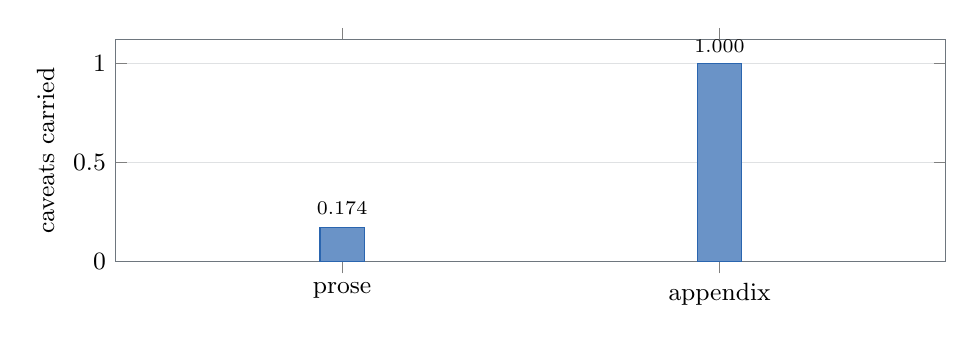
\begin{tikzpicture}
\begin{axis}[width=\textwidth,height=4.4cm,ybar,bar width=16pt,
  ymin=0,ymax=1.12,xtick={1,2},xticklabels={prose,appendix},
  ylabel={caveats carried},xmin=0.4,xmax=2.6,
  tick label style={font=\small},ylabel style={font=\small},
  axis line style={inkmut},ymajorgrids,grid style={inkmut!22}]
\addplot+[fill=accent!70,draw=accent] coordinates {(1,0.174) (2,1.000)};
\node[font=\scriptsize,anchor=south] at (axis cs:1,0.19) {0.174};
\node[font=\scriptsize,anchor=south] at (axis cs:2,1.005) {1.000};
\end{axis}
\end{tikzpicture}
\end{minipage}\hfill
\begin{minipage}{0.52\textwidth}
\centering
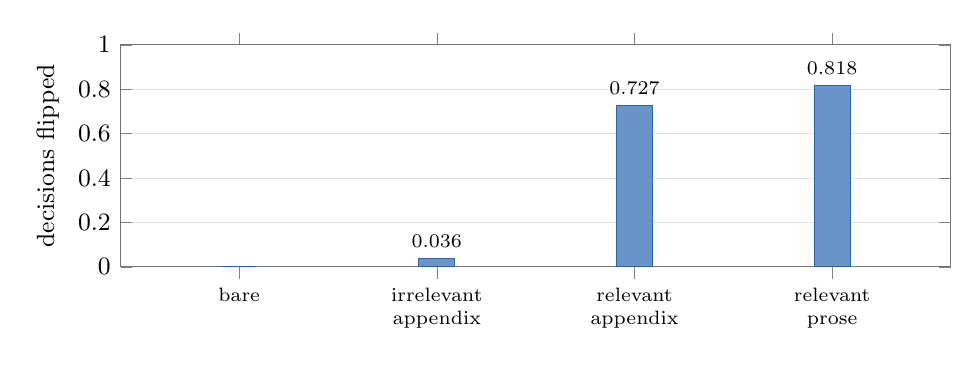
\begin{tikzpicture}
\begin{axis}[width=\textwidth,height=4.4cm,ybar,bar width=13pt,
  ymin=0,ymax=1.0,xtick={1,2,3,4},
  xticklabels={bare,{irrelevant\\appendix},{relevant\\appendix},
  {relevant\\prose}},xticklabel style={font=\scriptsize,align=center},
  ylabel={decisions flipped},xmin=0.4,xmax=4.6,
  tick label style={font=\small},ylabel style={font=\small},
  axis line style={inkmut},ymajorgrids,grid style={inkmut!22}]
\addplot+[fill=accent!70,draw=accent] coordinates
  {(1,0.000) (2,0.036) (3,0.727) (4,0.818)};
\node[font=\scriptsize,anchor=south] at (axis cs:2,0.045) {0.036};
\node[font=\scriptsize,anchor=south] at (axis cs:3,0.732) {0.727};
\node[font=\scriptsize,anchor=south] at (axis cs:4,0.823) {0.818};
\end{axis}
\end{tikzpicture}
\end{minipage}
\caption{The out-of-band channel, both halves. \textbf{Left}: share of
both-judge caveat sentences reaching the final artifact through writer
prose against the mechanically assembled appendix (byte-identical
prose in both arms). \textbf{Right}: share of registered two-token
reader decisions flipped by a planted decision-relevant caveat, by
delivery arm (11 items, 440 reads). Uptake is $+0.691$
\ci{+0.455}{+0.891} over the irrelevant-appendix control and at parity
with in-prose placement ($+0.091$ \ci{-0.036}{+0.218}).}
\label{fig:freight}
\end{figure*}

\subsection{Out-of-Band Channel}
\label{sec:res-channel}

The appendix delivers $1.000$ of both-judge caveat sentences against
the $0.174$ that survives prose transport, with the preference cost
not evaluable at power ($0.510$ \ci{0.267}{0.754}, $65/116$ ties). A
decision-relevant caveat delivered appendix-only flips a reader
model's registered two-token decision in $0.727$ of reads against
$0.036$ for the identical appendix block carrying an irrelevant caveat,
with direction-balanced items so that generic caution cannot
masquerade as uptake, and at parity with weaving the same sentence
into prose (Figure~\ref{fig:freight}). The channel that preference
judging cannot see changes decisions.

\subsection{Routed Re-consultation}
\label{sec:res-loop}

\textbf{Scripted replies.} Three arms over six planted tensions whose
deciding fact was withheld from round one: no clarification; a
length-matched clarification responsive in style but containing no
deciding fact; and the same clarification containing it. On runs where
the tension was named, the lead adopted the fact-implied resolution in
$7/7$ informed runs against $0.333$ in control (difference CI
\ci{+0.200}{+1.000}) and $0.200$ under the contentless clarification
(\ci{+0.545}{+0.947}). The information does the work rather than the
ritual, and the mechanism operates through the one capability the lead
demonstrably has, preference among overlapping sources, by
manufacturing an uncorrupted source at the contested quantity.

\textbf{Live seat.} Two further experiments replaced the scripted
reply with a real seat. The first buried the deciding fact in the
seat's own round-one contribution and halted at its registered pilot
gate, with the tension named in only $0.208$ of runs. The second
restored the original round-one bytes and supplied the fact only as
the seat's private working notes at reply time. The live seat conveyed
the fact in $21/21$ dispatched replies, and the lead adopted the
fact-implied resolution at $0.905$ against the archived control's
$0.333$ ($+0.571$ \ci{+0.139}{+0.912}), within $-0.095$
\ci{-0.227}{0.000} of the scripted ceiling. In $4/21$ live replies the
seat embellished the correctly conveyed fact with fabricated legal
authority and the lead adopted regardless; a registered follow-up
bounded the rate at $0.100$ \ci{0.047}{0.201} with the fact in hand
and $0.150$ \ci{0.081}{0.261} without it, concentrated on one trigger
topic ($15/20$ there, $0/100$ elsewhere) and name-stable across
samples, which licenses the blocklist filter.

\textbf{The trigger.} Table~\ref{tab:trigger} collects the three
consultation designs: each works when fired and fires rarely on
planted tensions. On organic inquiries the picture differs: in the
head-to-head experiment's 54 live pipelines, the orchestrator found a
role-named tension and dispatched on $0.85$ of runs.

\begin{table}[t]
\centering\footnotesize
\setlength{\tabcolsep}{4pt}
\begin{tabular}{lcc}
\toprule
 & When triggered & Trigger rate \\
\midrule
lead uses a clarification & $7/7$ & $0.34$ \\
seat routes a deferral & $0.909$ correct & $0.306$ \\
briefed seat conveys, live & $21/21$ conveyed & $0.208$ to $0.583$ \\
\bottomrule
\end{tabular}
\caption{Re-consultation is recognition-limited rather than
capability-limited, which is why the trigger is drawn from a mandated
artifact and never from self-assessment.}
\label{tab:trigger}
\end{table}

\subsection{Ablations and Rejected Components}
\label{sec:ablations}

\textbf{Isolation.} Making byte-fixed sibling contributions visible
under production prompts moved off-domain framework density by
$-0.009$ \ci{-0.048}{+0.028} against a pre-registered minimum
detectable difference of $+0.05$ to $+0.08$, with in-domain density
unchanged. The contamination rationale is withdrawn and the rule
stands on cost. A registered secondary measure pointed the other way
($-0.033$ \ci{-0.053}{-0.013} off-domain terms when siblings were
visible) and is recorded as a candidate mechanism, not claimed.

\textbf{Ownership routing map.} A stable, near-unanimous elicited map
of which seat owns each quantity, exactly the pattern a framework
would ship as a routing table, predicted arbitration at $0.500$ on
fresh items against $0.895$ descriptive, with a minimum detectable
difference of $0.68$. It is not in the harness.

\textbf{Prior plausibility.} A model's own plausibility rating
predicted which planted values it would adopt at $0.544$ and was
rejected as a boundary mechanism for redundancy.

\textbf{Content gate.} The rule that follow-up replies adding nothing
should be dropped failed two registered attempts on complementary
halves: a two-judge semantic gate passed vacuous fillers ($3/6$
dropped), and an extract-then-verify gate that fixed vacuity ($6/6$)
rejected $52\%$ of genuine live replies. Under the frozen commitment
there is no third attempt without purpose-built labeled data; the
deployed posture is flagged delivery. The fabrication blocklist, by
contrast, validated at $21$ true hits, $0$ false positives, and $0$
misses over the $141$-reply archive and is deployed.

\subsection{Generalization}
\label{sec:generalization}

Three results extend beyond the conditions that produced them. The
preference lift and the form-Y penalty replicate under a judge from a
disjoint model family (Section~\ref{sec:pref}). The transport slope
replicates on an extension corpus of nine cases the original corpus
never contained, for both writers (Figure~\ref{fig:transport}). And
the trigger scarcity measured on planted tensions ($0.208$ to $0.583$)
gives way to $0.85$ dispatch on organic inquiries, so the harness's
coverage bound on natural problems is set by the identification rate
of Equation~\ref{eq:protection} rather than by the trigger.

\section{Head-to-Head Preference Evaluation}
\label{sec:headtohead}

With every mechanism separately verdicted, the remaining question was
whether the assembled harness costs anything on the recipe's own
metric. The harness's final artifact was judged against the unmodified
pipeline's under Equation~\ref{eq:pref} with two judge families ($108$
pairs). The result is no evaluable difference: primary-judge share
$0.562$ \ci{0.375}{0.765}, replication $0.333$ \ci{0.083}{0.562}, both
spanning $0.5$, with large effects excluded in both directions. The
harness's preference standing is inherited from aggregation, which
both artifacts share; its mechanisms were never preference plays, and
shipping them (five caveats per artifact, a follow-up round,
restructured seats) costs nothing detectable. The appendix's
within-pair attribution is mildly positive ($+0.073$ toward the
harness).

The null is the correct outcome rather than a shortfall. Preference
judging at this scale is majority reading-order, penalizes visible
caution, and cannot see whether a caveat reached the reader or whether
a corrupted value was adopted. The failures the harness fixes are, by
construction, invisible to the metric the recipe reports.

\section{Related Work}
\label{sec:related}

\textbf{Aggregation pipelines.} MoA \cite{wang2024moa} is the recipe
this paper hardens. Li et al.\ \cite{li2025selfmoa} showed that
aggregating repeated samples of the single best model outperforms
mixed MoA on AlpacaEval, converging from the benchmark side with the
per-model signature result of Section~\ref{sec:signature}. Wang et
al.\ \cite{wang2024rebuttal} report that a single strongly prompted
agent can match multi-agent discussion, consistent with the finding
that the one retained intervention routes information rather than
deliberation.

\textbf{Judge pathologies.} Position and verbosity bias in LLM judges
\cite{zheng2023judging}, length correlations under preference
optimization \cite{singhal2023length}, and sycophancy under preference
pressure \cite{sharma2023sycophancy} motivate the order-debiased
two-family protocol and sharpen into the measured phrase penalty of
Section~\ref{sec:pref}.

\textbf{Instruction following and pre-registration.} The phrase-swap
design is, to the author's knowledge, the first to test an epistemic
instruction by swapping its named surface form under otherwise
byte-identical prompts. No prior work is known that pre-registers each
component of a multi-agent architecture and reports the failures
alongside the survivals. The complete registration ledger, every
deviation and verdict, and the measurement kit are released with the
project repository (Appendix~\ref{app:details}).

\section{Conclusion}
\label{sec:conclusion}

The Mixture-of-Agents recipe delivers a preference lift and rests on a
mechanism story its evaluation never tests. Tested under
pre-registration at auditable scale, the story fails: the aggregator
selects rather than verifies, instructions install phrases that judges
penalize, prose loses most of the qualification it is given, and
self-assessment predicts behavior at chance. The harness presented here
accepts the recipe's structure and lift, adds five mechanisms each
licensed by one of those failures, and submits every mechanism to a
prospective test with the kill condition written first. The mechanisms
that survived did so with causal or predictive effect sizes; two
rationales were demoted, one candidate rule was rejected, one gate is
recorded as not deployable, and the assembled harness is
indistinguishable from the recipe on the recipe's own metric. That is
the hardening the paper proposes: not a better score, but a pipeline
whose every component can say which experiment it survived.

\section*{Impact Statement}

This work concerns the reliability of multi-agent language model
pipelines in advisory settings, where a corrupted input adopted without
verification or a caveat lost in synthesis can reach a decision maker.
The harness is intended to reduce both failure modes and to make their
residual rates measurable in deployment. The findings on preference
judging carry a caution for evaluation practice: single-ordering
LLM-judge comparisons at the studied scale predominantly measure
reading order, and preference-trained pipelines can be expected to
shed visible epistemic marking. All experiments used open models on
local hardware with synthetic advisory scenarios; no human subjects or
personal data were involved. Results are bounded to 7 to 20B models,
advisory-domain English, and small case counts, and should be retested
at larger scale before being relied on in deployment.

\begin{thebibliography}{9}
\bibitem{wang2024moa} J.~Wang, J.~Wang, B.~Athiwaratkun, C.~Zhang,
J.~Zou. Mixture-of-Agents enhances large language model capabilities.
\emph{arXiv:2406.04692}, 2024.
\bibitem{li2025selfmoa} W.~Li et al. Rethinking Mixture-of-Agents: is
mixing different large language models beneficial?
\emph{arXiv:2502.00674}, 2025.
\bibitem{zheng2023judging} L.~Zheng et al. Judging LLM-as-a-judge with
MT-Bench and Chatbot Arena. \emph{NeurIPS Datasets and Benchmarks},
2023.
\bibitem{singhal2023length} P.~Singhal et al. A long way to go:
investigating length correlations in RLHF. \emph{arXiv:2310.03716},
2023.
\bibitem{sharma2023sycophancy} M.~Sharma et al. Towards understanding
sycophancy in language models. \emph{arXiv:2310.13548}, 2023.
\bibitem{wang2024rebuttal} Q.~Wang et al. Rethinking the bounds of LLM
reasoning: are multi-agent discussions the key?
\emph{arXiv:2402.18272}, 2024.
\end{thebibliography}

\appendix

\section{Supplementary Discussion}
\label{app:charter}

\textbf{The Goodhart charter.} The following quantities are
diagnostics and may not be optimization targets. \emph{Trigger rate}:
raising it blindly manufactures the contentless-consultation condition
of Section~\ref{sec:res-loop}, in which a length-matched reply with no
deciding fact moved adoption to $0.200$. \emph{Hedge counts and
compliance shares}: raising them produces the dictated phrase of
Section~\ref{sec:phrase}, which Section~\ref{sec:pref} shows judges
penalize. \emph{Transport slope}: optimizing it against the writer's
own text rewards invented qualification, which the writer already
produces at $0.333$ on inputs containing none. \emph{Preference score on
epistemic content}: the instrument is majority reading-order and
penalizes visible caution. The optimizable signal must live outside
the pipeline's own text, in verified outcomes where ground truth
exists.

\textbf{Operating economics.} Everything downstream of the trigger is
measured and works. On planted tensions the trigger fires at $0.208$
to $0.583$ by batch; on organic inquiries dispatch fired on $0.85$ of
pipelines. Sibling isolation saves approximately $10$k input
characters and $14\%$ output length per seat. The harness's telemetry
doubles as a replication battery: every deployment yields transport
estimates, trigger telemetry, phrase-swap slots for proposed
instructions, and preference-versus-verified divergence wherever
ground truth exists, each with its attainability gate.

\textbf{Open risks.} Per-item protection is bimodal with the boundary
mechanism unknown after two rejected candidates. The fabrication bound
covers adversarial case citations on one trigger topic only, and the
seat never admits the gap ($0/20$ sampled), so the bound is a floor
rather than a ceiling on confabulation. The preference cost of the
appendix is bounded but not evaluable at current power. The pipeline
used no tool calling or retrieval, and the paper makes no claim about
how those would interact with the harness.

\section{Experimental Details}
\label{app:details}

\textbf{Phrase-swap.} 18 cases, 7 repeats, 378 runs. Treated clause:
``When you state a number that is an estimate rather than an
established fact, label it using the phrase `modeled at' '' (form X)
or ``\ldots `taken to be' '' (form Y). Form X: 11 registry entries
across 9 prompt symbols. Form Y: zero archive occurrences; spontaneous
rate $0/249$ clean-provenance runs for both forms. Emission $43.7$ to
$46.6$ sentences per run across arms. A harness gate refused to run
unless each arm contained exactly its own form and no other registry
phrase.

\textbf{Preference.} 126 pairs per comparison, both orderings, decisive
only when the same side wins both. Primary judge \texttt{gpt-oss:20b};
replication judge a 30B Qwen3 MoE selected from three candidates on
parse and decisive rates only. Decisive counts: 44, 46, 41 (primary);
33, 29, 23 (replication). Arm mean lengths 7{,}757 against 7{,}649
characters for the lift comparison.

\textbf{Source selection.} 27 runs per arm; planted arithmetic errors;
exact match on known values. Single-factor redundancy experiment:
corrupted adoption $0.900$ (sole-sourced) against $0.450$ (second seat
assigned); clean adoption $0.000$ against $0.500$.

\textbf{Transport.} 144 runs, 18 cases, two writers
(\texttt{gpt-oss:20b}, \texttt{phi4:14b}), two corpora (original, 9
cases; extension, 9 new cases). Supply is judge-measured with
inter-judge $r = 0.528$; correcting for attenuation on the original
corpus moves $0.150$ to $0.217$.

\textbf{Seating gate.} Ten candidates; two screen items disjoint from
the pipeline case set; $800$ visible-character degeneracy threshold;
verdicts committed before any pipeline run.

\textbf{Planner.} Identification against analyst-authored labels on
the case battery; assignment over 40 plans; live conveyance across
briefed seats; end-to-end clean adoption on the pipeline cases.

\textbf{Out-of-band channel.} Carriage: byte-identical prose in both
arms, appendix assembled from both-judge caveat sentences; preference
$65/116$ ties. Uptake: 18 authored items, 11 retained after a
registered floor gate, 440 reads, direction-balanced (blocking and
enabling caveats), two-token reader decisions.

\textbf{Re-consultation.} Six planted tensions; conditioned $n$ of
seven in the scripted decisive cell; judge agreement $0.703$ on the
analysis population and $0.583$ overall, both reported. Live cells
compare against archived arms under a registered, never-pooled
fresh-batch check. Fabrication follow-up: 20 replies with the fact in
hand, 100 elsewhere.

\textbf{Head-to-head.} 108 pairs; 54 live harness pipelines; two judge
families; order-debiased.

\section{Instrument Validation}
\label{app:instruments}

Fourteen instrument-validity findings are recorded in the ledger. The
three that bear on this paper: (i) entanglement, exposed by a
pattern-level decomposition in which an instruction moved dictated
phrasings from $0/30$ to $28/30$ and non-dictated phrasings of the same
construct from $1/30$ to $4/30$ (difference-in-differences $+0.83$
\ci{+0.67}{+1.00}); (ii) the dictation registry, 125 entries from 35
prompt symbols by AST parsing and quote scanning, which on its first
run found an earlier judge prompt enumerating the seven phrases the
writing prompts dictated, and whose measured over-attribution is zero
across 2{,}907 spans (438{,}797 characters) and 60 de-scaffolded runs;
and (iii) reading-order dominance, with raw first-position preference
of $0.85$ to $0.88$ across a 20B MoE, a 30B MoE, a 14B dense model, and
a 7B dense model, and decisive rates of $0.05$ to $0.40$ after
debiasing. Document-level construct judging scored $0.622$ agreement
against $0.910$ for the sentence-level protocol and was rejected.

\end{document}
